\chapter{Experimentelle Evaluation}
\label{chap:experimente}

\section{Aufbau Demonstrationssysteme}
Simulation und theoretische Evaluation für Robotik nicht zielführend.
Daher mehrere mobile Manipulatoren gebaut und praxisnah getestet. 
Gemeinsamkeit: Hohe Anzahl an Freiheitsgraden, Kinematik erzeugt sehr wandelbare Geometrien.
Approximation über 2D Projektion nicht umsetzbar.

\begin{figure}[hbtp]
	\centering
	\begin{subfigure}[t]{0.33\textwidth}
		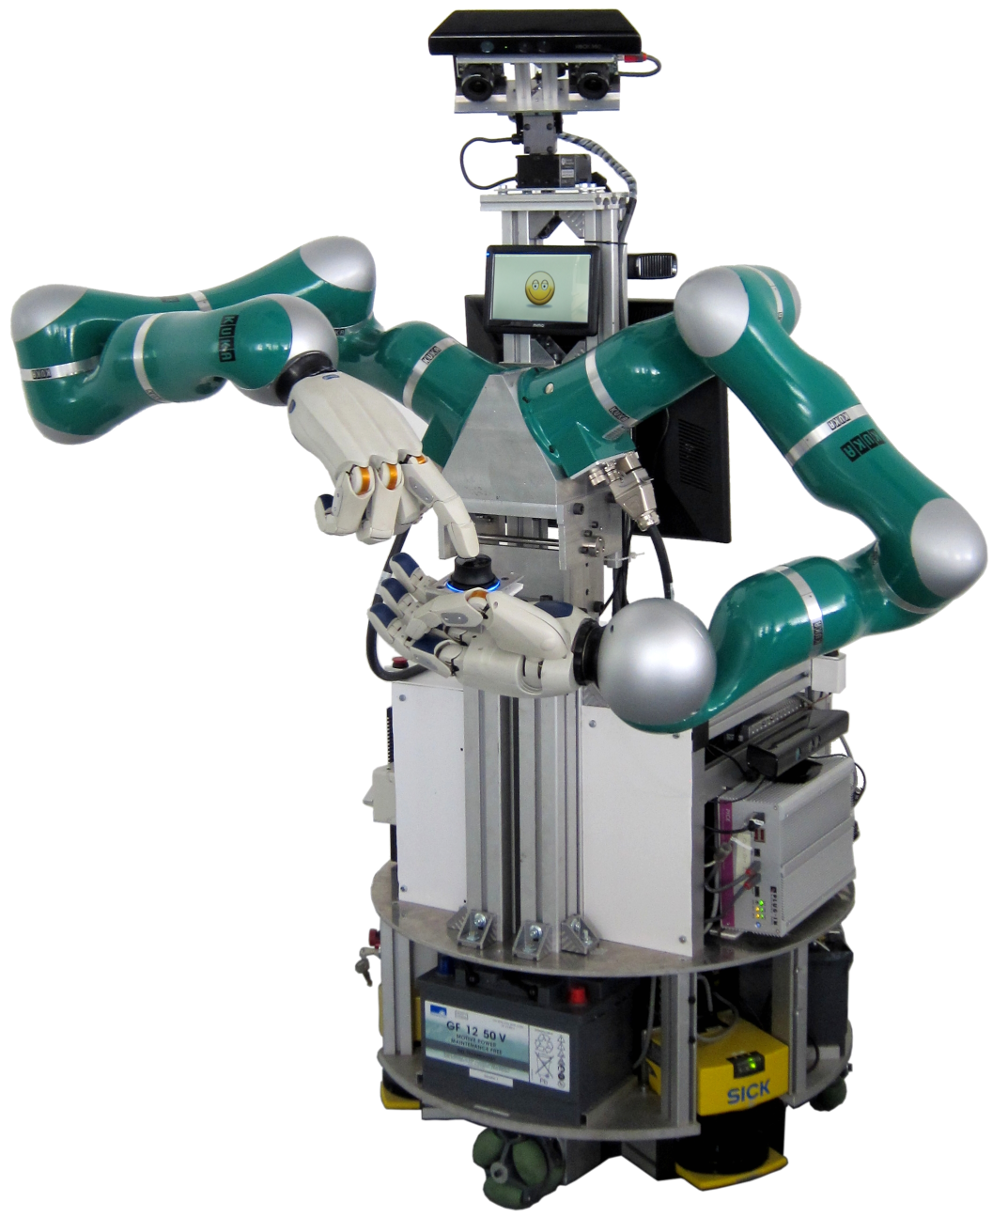
\includegraphics[width=\textwidth]{04_images/robots/Adero.png}
		\caption{Adero}
		\label{subfig:Adero}
	\end{subfigure}
	\begin{subfigure}[t]{0.28\textwidth}
		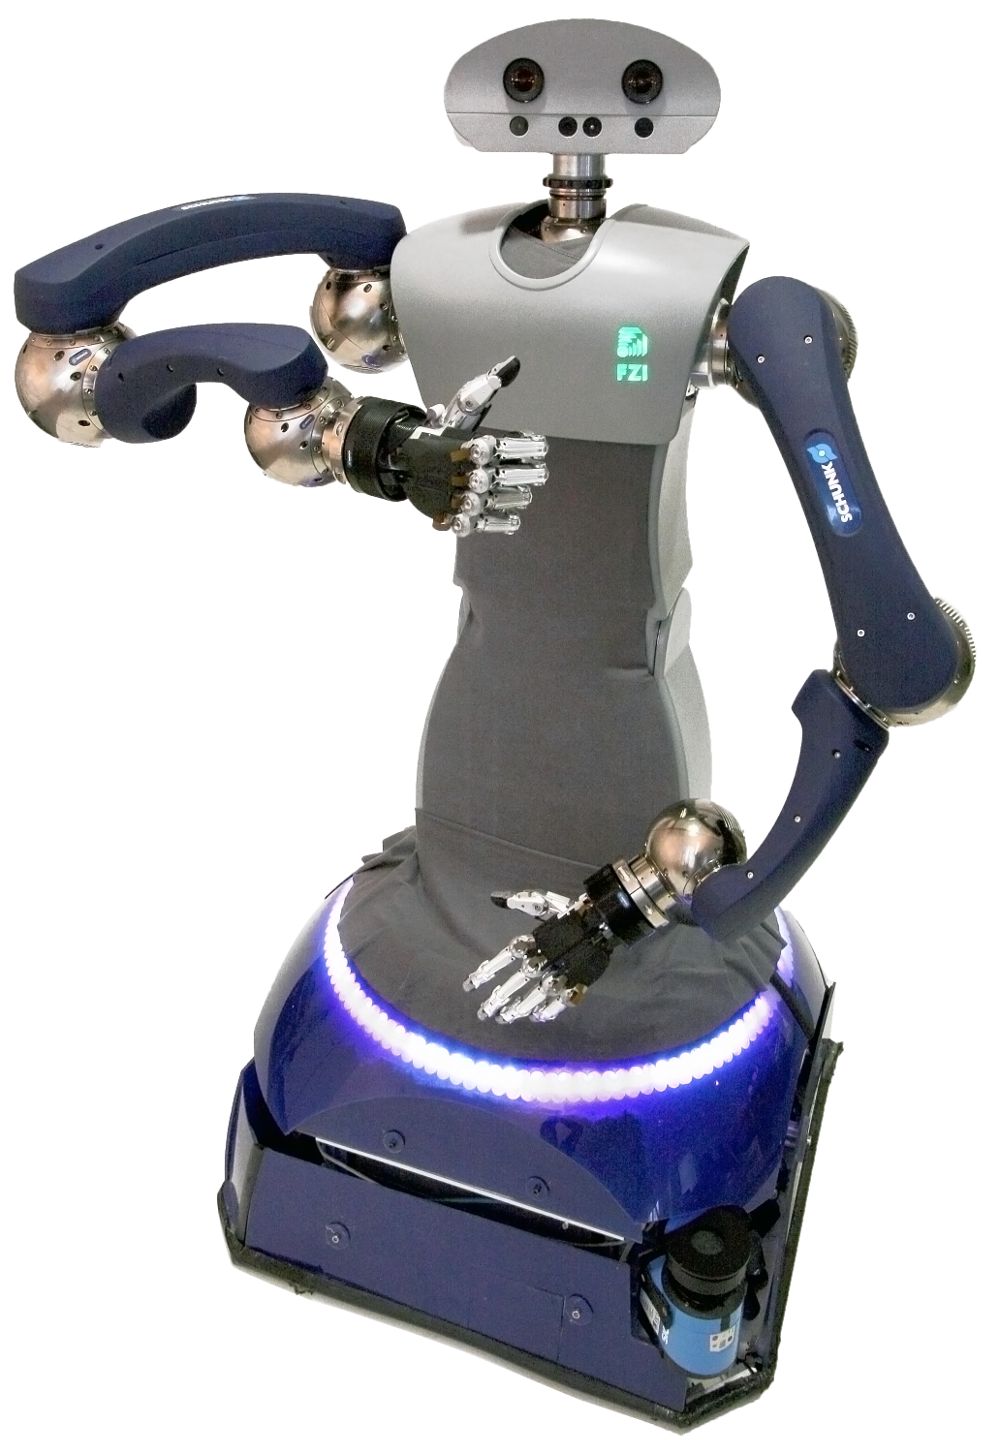
\includegraphics[width=\textwidth]{04_images/robots/HoLLiE.png}
		\caption{HoLLiE}
		\label{subfig:HoLLiE}
	\end{subfigure}
	\begin{subfigure}[t]{0.29\textwidth}
		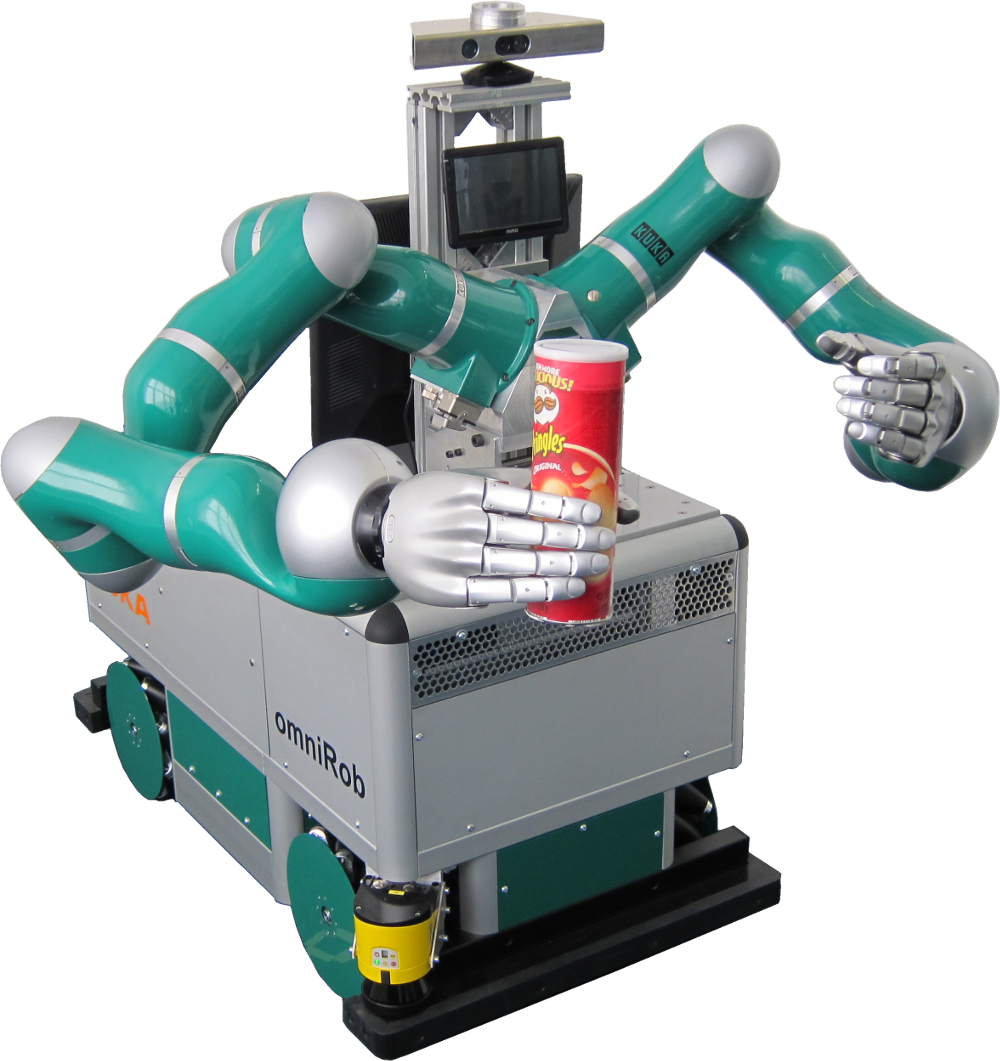
\includegraphics[width=\textwidth]{04_images/robots/IMMP.png}
		\caption{IMMP}
		\label{subfig:IMMP}
	\end{subfigure}
	\caption{Demonstratorsysteme, deren Entwicklung der Autor im Laufe der Dissertation leitete:
		Anthropomrphe mobile Manipulationsplattform Adero, House of Living Labs intelligent Escort (HoLLiE),
		Industrielle Mobile Manipulations Plattform (IMMP)}
	\label{fig:own_robots}
\end{figure}



\begin{algorithm}[ht]
	\caption{\label{alg:pre_optimizer}Local Grasp Optimizer}
	\begin{algorithmic}[1]
		\REQUIRE ~\\
		O : Pointcloud of object surface \\ 
		H : Swept-Volume of grasp \\ 
		P : Particle defining initial $(x,y)$, $(\alpha,\beta,\gamma)$ pose of the object in hand
		\ENSURE ~\\
		
		$\vec{\varphi}_{\text{best}}$ : Finger joint angles for best grasp \\
		P: Contains object pose for best grasp
		
		\STATE O $\leftarrow$ transform(O, P)\hfill $\setminus\setminus$ Place object at initial pose
		\STATE O $\leftarrow$ transform(O, y-start)\hfill $\setminus\setminus$ Stick object into hand
		
		\FOR{xz-shift $\leftarrow$ -max-shift \TO max-shift}
		\FOR[\hfill $\setminus\setminus$ Move object out of hand]{y-shift $\leftarrow$ 0~mm \TO $200~\textnormal{mm}$}
		\STATE offset $\leftarrow$ xz-shift + y-shift
		\STATE num-colls $\leftarrow$ collisionCheckOffset(O, H, offset)
		\IF{num-colls $==$ 0}
		\STATE $\vec{\varphi}$, $\sharp$colls $\leftarrow$ sweptCollisionCheck(O, H, offset)
		\IF{$\sharp\text{colls} > \sharp\text{colls}_\text{best}$  }
		\STATE \hfill $\setminus\setminus$ Local optimum found
		\STATE $\sharp\text{colls}_\text{best} \leftarrow \sharp\text{colls}$
		\STATE $\text{pose}_\text{best} \leftarrow$ offset
		\STATE $\vec{\varphi}_{\text{best}}$ $\leftarrow$ $\vec{\varphi}$
		\ENDIF
		\ENDIF
		\ENDFOR
		\ENDFOR
		\RETURN P, $\vec{\varphi}_{\text{best}}$
	\end{algorithmic}
\end{algorithm}
\change{Code aktualisieren!}